\documentclass[12pt]{article} % use larger type; default would be 10pt
\usepackage[czech]{babel}
\usepackage[utf8]{inputenc} % set input encoding (not needed with XeLaTeX)

%%% PAGE DIMENSIONS
\usepackage{geometry} % to change the page dimensions
% \usepackage[left=2cm,right=2cm,top=2cm,bottom=2cm]{geometry}
\geometry{a4paper}
% \geometry{margin=2in} % for example, change the margins to 2 inches all round
% \geometry{landscape} % set up the page for landscape

\usepackage{graphicx} % support the \includegraphics command and options
\usepackage{wrapfig} % support the wrapfigure section

\usepackage{tikz} % graphs
\usepackage{pgfplots}

\usepackage{hyperref} % links in \tableofcontents
\hypersetup{
	colorlinks,
	citecolor=black,
	filecolor=black,
	linkcolor=black,
	urlcolor=black
}

% \usepackage[parfill]{parskip} % Activate to begin paragraphs with an empty line rather than an indent

%%% PACKAGES
\usepackage{booktabs} % for much better looking tables
\usepackage{array} % for better arrays (eg matrices) in maths
% \usepackage{paralist} % very flexible & customisable lists (eg. enumerate/itemize, etc.)
\usepackage{verbatim} % adds environment for commenting out blocks of text & for better verbatim
\usepackage{subfig} % make it possible to include more than one captioned figure/table in a single float
% These packages are all incorporated in the memoir class to one degree or another...
\usepackage{float}

%%% HEADERS & FOOTERS
\usepackage{fancyhdr} % This should be set AFTER setting up the page geometry
\pagestyle{fancy} % options: empty , plain , fancy
\renewcommand{\headrulewidth}{0pt} % customise the layout...
\lhead{}\chead{}\rhead{}
\lfoot{}\cfoot{\thepage}\rfoot{}

%%% SECTION TITLE APPEARANCE
\usepackage{sectsty}
\allsectionsfont{\sffamily\mdseries\upshape} % (See the fntguide.pdf for font help)
% (This matches ConTeXt defaults)

%%% ToC (table of contents) APPEARANCE
\usepackage[nottoc,notlof,notlot]{tocbibind} % Put the bibliography in the ToC
\usepackage[titles,subfigure]{tocloft} % Alter the style of the Table of Contents
\renewcommand{\cftsecfont}{\rmfamily\mdseries\upshape}
\renewcommand{\cftsecpagefont}{\rmfamily\mdseries\upshape} % No bold!
\newcommand{\bigsize}{\fontsize{35pt}{20pt}\selectfont}

%%% END Article customizations

\begin{document}
\begin{titlepage}
	
\includegraphics[scale=0.7]{logo.jpg}
	\vspace*{\fill}
	\begin{center}
		\textsc{\LARGE \bigsize Měření impedance voltmetrem, ampérmetrem a wattmetrem}\\[1cm]
		Martin Zlámal \\[1cm]
		{\small\em \copyright \ Datum poslední revize \today } \\
		\LaTeX
	\end{center}
	\vspace*{\fill}
\end{titlepage}
\tableofcontents
\listoffigures
\listoftables
\newpage

\section{Zadání}
\begin{enumerate}
\item Pomocí voltmetru, ampérmetru a wattmetru změřte závislosti $L=f(I)$ a $R=f(I)$
pro danou cívku s jádrem.
\item Odvoďte vztahy pro paralelní náhradu měřené impedance.
\end{enumerate}

\section{Teoretický úvod}
\begin{description}
\item[Metody měření impedancí] \hfill \\
Impedanci měříme při střídavém proudu, aby nedošlo pouze ke změření činné složky impedance. Měřiti můžeme například voltmetrem, ampérmetrem a wattmetrem, což je způsob řešení v této práci, nebo pomocí tří ampérmetrů, popř. voltmetrů. Impedance se dají také měřit číslicově případně můstkem.
\item[Náhradní zapojení cívky] \hfill \\
Náhradním zapojením cívky myslíme zapojení ideální cívky do série s s odporem vlastního vinutí. V takovém případě je $Z=R+jX_L=R+j\omega L$. Velikost impedance je v tomto případě $|Z|=\sqrt{R^2 + \omega^2 L^2}$ (Pythagorova věta). Pro případ zapojení ideální cívky paralelně k odporu vlastního vinutí by platilo, že $Z=\frac{jX_L\cdot R}{jX_L+R}=\frac{j\omega RL}{R+j\omega L}$. V takovém případě je velikost impedance $|Z|=\frac{|\omega RL|}{\sqrt{R^2 + \omega^2 L^2}}$ což je obyčejná absolutní hodnota.
\end{description}

\section{Schéma zapojení}
\begin{figure}[H]
\center
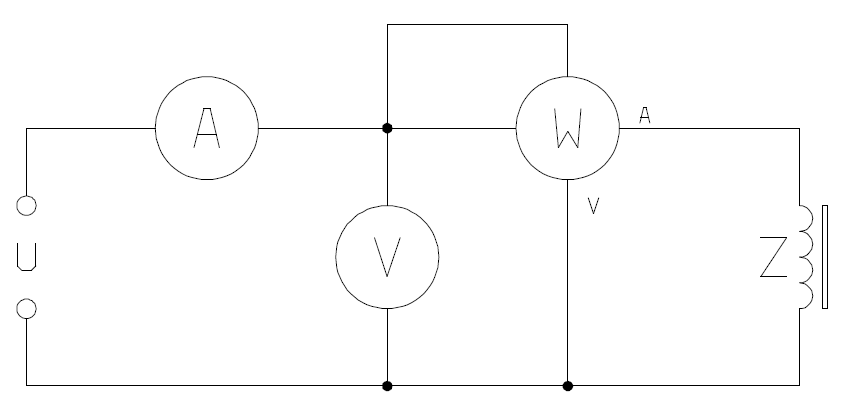
\includegraphics[scale=0.5]{schema.png}
\caption{Schéma zapojení}
\end{figure}
Výše uvedené schéma je schválně vzorové. K měření byl použit jeden přístroj, který kombinoval všechny měřící přístroje dohromady. Nicméně výsledné schéma by bylo poněkud nevypovídající.

\section{Postup měření}
Obvod zapojíme podle schématu. Nepoužíváme však tři přístroje, ale pouze jeden, který všechny přístroje kombinuje. Na autotransformátoru nastavuje napětí rovnoměrně v rozsahu $0-240V$ a odečítáme proud a výkon. Následně spočteme impedanci, činný odpor, reaktanci a indukčnost cívky podle níže uvedených vzorců.

\section{Naměřené a dopočítané hodnoty}
\captionof{table}{Naměřené a dopočítané hodnoty}
\begin{tabular}{|c|c|c|c|c|c|c|}
\hline 
$U[V]$ & 30 & 90 & 120 & 160 & 200 & 240 \\ 
\hline 
$I[A]$ & 0,009 & 0,020 & 0,025 & 0,032 & 0,038 & 0,045 \\ 
\hline 
$P[W]$ & 0,066 & 0,520 & 0,860 & 1,390 & 2,020 & 2,730 \\ 
\hline 
$Z[\Omega]$ & 3333,3 & 4500 & 4800 & 5000 & 5263,2 & 5333,3 \\ 
\hline 
$R[\Omega]$ & 814,8 & 1300 & 1376 & 1357,4 & 1398,9 & 1348,2 \\ 
\hline 
$X[\Omega]$ & 3232,2 & 4308,1 & 4598,6 & 4512,2 & 5073,9 & 5160,1 \\ 
\hline 
$L[H]$ & 10,23 & 13,71 & 14,64 & 15,32 & 16,15 & 16,43 \\ 
\hline 
\end{tabular}
\linebreak \\\\
Velikost impedance spočteme podle vzorce:
\begin{equation}
Z = \frac{U}{I} = \frac{90}{0,02} = 4500 \Omega
\end{equation}
Následně využijeme vzorce pro činný odpor cívky:
\begin{equation}
R = \frac{P}{I^2} = \frac{0,52}{0,02^2} = 1300 \Omega
\end{equation}
Pro reaktanci cívky využijeme vzorce:
\begin{equation}
X = \sqrt{\left(\frac{U}{I}\right)^2-\left(\frac{P}{I^2}\right)^2} = \sqrt{\left(\frac{90}{0,02}\right)^2-\left(\frac{0,52}{0,02^2}\right)^2} = 4308,1 \Omega
\end{equation}
Díky znalosti reaktance cívky můžeme snadno spočítat indukčnost cívky:
\begin{equation}
L = \frac{X}{2\pi f} = \frac{4308,1}{2\pi 50} = 13,71 H
\end{equation}

\section{Grafy}
\begin{figure}[H]
\centering
	\begin{tikzpicture}
		\begin{axis}[
			width=1\textwidth,
	      	height=0.5\textwidth,
			xlabel={$I$},
			ylabel={$L$}]
		\addplot[color=red,mark=x] coordinates {
			(0.009,10.23)
			(0.020,13.71)
			(0.025,14.64)
			(0.032,15.32)
			(0.038,16.15)
			(0.045,16.43)
		};
		\addlegendentry{$L=f(I)$}
		\end{axis}
	\end{tikzpicture}
	\caption{Závislost $L=f(I)$}
\end{figure}

\begin{figure}[H]
\centering
	\begin{tikzpicture}
		\begin{axis}[
			width=1\textwidth,
	      	height=0.5\textwidth,
			xlabel={$I$},
			ylabel={$R$}]
		\addplot[color=red,mark=x] coordinates {
			(0.009,814.8)
			(0.020,1300)
			(0.025,1376)
			(0.032,1357.4)
			(0.038,1398.9)
			(0.045,1348.2)
		};
		\addlegendentry{$R=f(I)$}
		\end{axis}
	\end{tikzpicture}
	\caption{Závislost $R=f(I)$}
\end{figure}

\newpage

\section{Závěr}
V měření bylo ověřeno, že impedance je skutečně složena z reální části (R) a (X), což odpovídá geometrickému součtu těchto hodnot ($Z=\sqrt{R^2+X^2}$). To také odpovídá vzorci pro výpočet impedance ze sériového náhradního zapojení ($|Z|=\sqrt{R^2+\omega^2L^2}$). Odvození viz teoretický úvod. Z grafů pak lze vyčíst, že se vzrůstajícím proudem narůstá také hodnota indukčnosti cívky a činný odpor cívky. U cívky s feromagnetickým jádrem indukčnost s proudem nejprve vzrůstá ke svému maximu (pro proud, při kterém weber-ampérová charakteristika závislosti magnetického indukčího toku v cívce na protékajícím proudu má tečnu procházející počátkem) a poté klesá.

\section{Přístroje}
\begin{itemize}
\item Multimetr HM S115-2 Hanes, evid. 178687
\item Autotransformátor METREL 0-260V, 50-400Hz, evid. 181390
\item Cívka s jádrem
\end{itemize}

\end{document}
